\section{System instructions}
\label{app:system_instructions}
In order to run the core system the following dependencies are required:
\begin{itemize}
\item Python 2.7
\item Theano
\item Numpy
\item Unirest
\item Python Imaging Library (PIL)
\end{itemize}

The system has only been tested with Ubuntu 14.04, but it should be possible to run on both Windows and Linux as long as the listed dependencies have been installed. Ubuntu is highly recommended because of a more convenient installation process. \\

A Nvidia GPU is also highly recommended for running the system. In most instances a GPU can give considerable speed improvements when training compared to a CPU. This is critical when having to deal with large datasets and models with millions of parameters. In order for Theano to efficiently use your GPU while training, CUDA Toolkit has to be installed. \\

A graphical user interface can also be utilized for monitoring the training. Running experiments can be stopped from this user interface, as well as a debugging option which display examples and model predictions. In addition all experiment data and results are stored as JSON, and can be viewed in the user interface. This includes, a loss per epoch plot, precision and recall curve and hyperparameters configuration. \\

The monitoring system can either be run locally, or installed on a server. All communication between the core system and the monitoring system is done by HTTP messaging. To enable monitoring, {\it enable\_gui} should be set to true in the core system's config file. Furthermore, the url to the monitoring system's api must also be set for the {\it endpoint} parameter. in  Utilizing this monitoring system requires these dependencies:
\begin{itemize}
\item Node.js
\item MongoDB
\end{itemize}

For installation instructions, please read the included README files of the repositories. The URL of these repositories are listed below:

\begin{itemize}
\item https://github.com/olavvatne/CNN
\item https://github.com/olavvatne/ml-monitor
\end{itemize} 

\section{Experiment tools overview}
\label{app:tools}
All tools which have been created for this thesis are listed below. The source code can be found inside the tools module of the road detection system's repository.
\begin{itemize}
\item measurement.precisionrecall.py\\
The tool creates the precision and recall curve. Command line options can be supplied.
\item layer.visualize.py\\
Opens a params.pkl file, containing the weights and hyperparameter configuration of a trained network. It creates a visualization of the kernels in the network's input layer.
\item distribution.curriculum\_diff.py\\
Samples patch examples and creates a histogram showing the patch dataset difficulty estimate distribution. Useful for setting the  threshold $D_\theta$ when conducting experiments. Also useful for verifying the content in a curriculum patch dataset stage.
\item distribution.dataset\_std.py\\
Tool for finding an estimate of a dataset's standard deviation. This value is used by the contrast normalization in the pre-processing step.
\item distribution.label\_dist\\
Counts the percentage of true label pixels in a dataset with binary labels.
\item curriculum.dataset\_create.py\\
Tool for pre-generating a curriculum patch dataset. Command line options can be supplied to, select a teacher, the thresholds $D_\theta$, the teacher's optimal threshold value, and dataset. The tool also comes with a baseline option which generate a staged patch dataset without curating the content of each stage.
\item convert.alpha.py\\
Converts a RGB dataset to RGBA. A quirk of the Python module PIL makes RGBA preferable when rotating an images. Areas not covered by pixels after a rotation, aare set to transparent with RGBA. With RGB, these pixels are set to black, which results in a lot of patch examples with no content.
\item figure.average\_compare.py\\
Averages experiment runs, and plots the averaged MSE loss and precision and recall curve from the test dataset. The tool also marks the precision and recall breakeven point for each plot. The resulting figures are used for comparison purposes in this thesis.
\item figure.average\_loss.py\\
Averages the test, validation and training loss from experiment replicates, and plots the result in a loss per epoch plot. 
\item figure.average\_noise\_levels\\
Averages the final epoch's test loss of an experiment. It also averages the precision and recall breakeven of each replicate experiment. The figures created by this tools, show the MSE loss and breakeven point, over increasing levels of label noise.
\end{itemize}

\section{Experiment Population Normality Assumption}
\label{app:normality}
The Welch's t test assumes that the samples are independent, and drawn from an approximately normal distributed population. In this appendix, the assumption of normality is explored further.\\

One way of verifying that a population do not violate the normality assumption is to create a normal Q-Q plot. These plots plot each sample based on its quantile and the corresponding theoretical quantile expected from a normal distribution. The population samples are normally distributed if the plotted points approximately fit a 45 degree line. The normal Q-Q plots comparing the test loss populations of {\it Experiment E1 - 0\% omission noise} to normal distributions can be found in Figure \ref{fig:normality_baseline} and Figure \ref{fig:normality_bootstrapping}. The plots are clearly affected by sample variability caused by the small sample sizes. This can be seen in Figure \ref{fig:normality_random}, where samples randomly picked from a normal distribution are plotted.  This plot is created from 10 randomly drawn samples of a normal distribution with mean and variance equal to that of the baseline population. Figure \ref{fig:normality_random100} displays the normal Q-Q plot of 100 random samples drawn from a normal distribution. This plot fits the line more closely than \ref{fig:normality_random}. Because of the small sample sizes, it can be hard to confidently assess whether the experiment populations are normally distributed or not.  \\

\begin{figure}
\begin{subfigure}{0.38\textwidth}
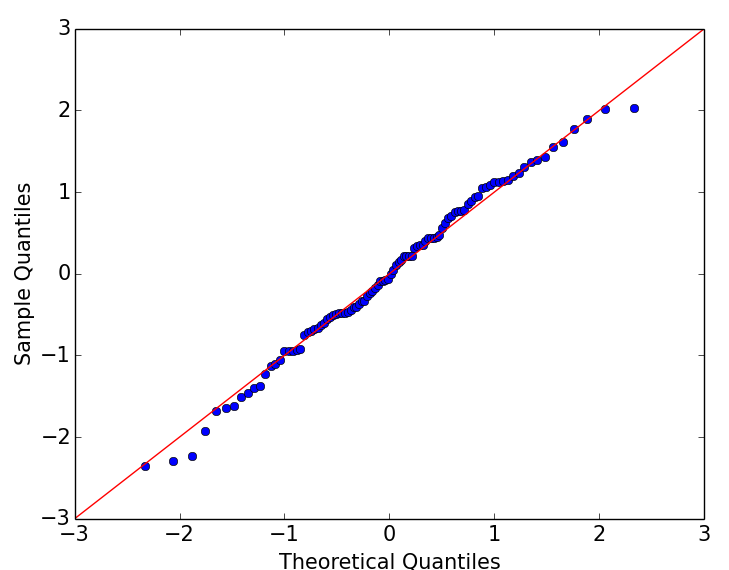
\includegraphics[width=\linewidth]{figs/normality/100samples_random2.png}
\caption{100 samples from a normal distribution} \label{fig:normality_random100}
\end{subfigure}
\hspace*{\fill} % separation between the subfigures
\begin{subfigure}{0.38\textwidth}
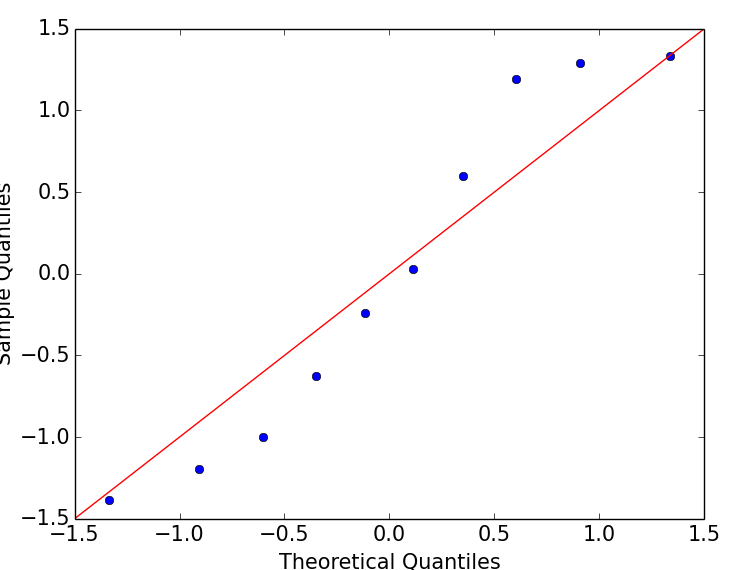
\includegraphics[width=\linewidth]{figs/normality/10samples_random2.png}
\caption{10 samples from a normal distribution} \label{fig:normality_random}
\end{subfigure}

\begin{subfigure}{0.38\textwidth}
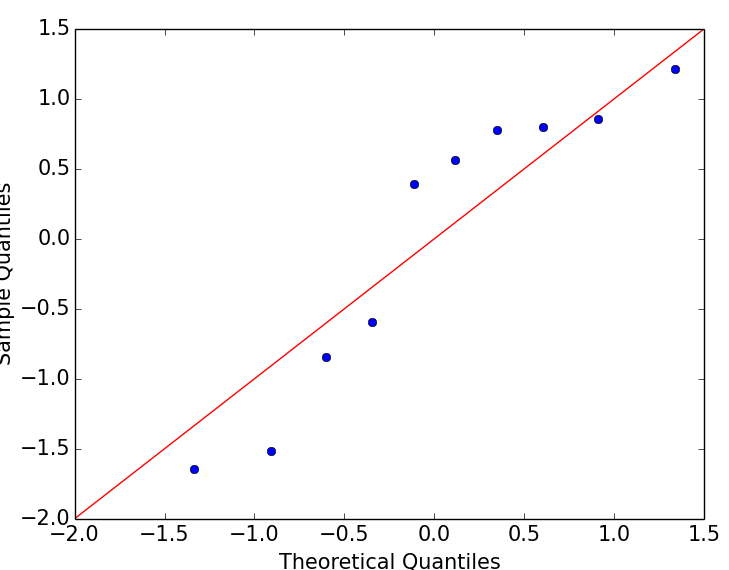
\includegraphics[width=\linewidth]{figs/normality/10samples_baseline2.png}
\caption{Baseline samples from Experiment E1} \label{fig:normality_baseline}
\end{subfigure}
\hspace*{\fill} % separation between the subfigures
\begin{subfigure}{0.38\textwidth}
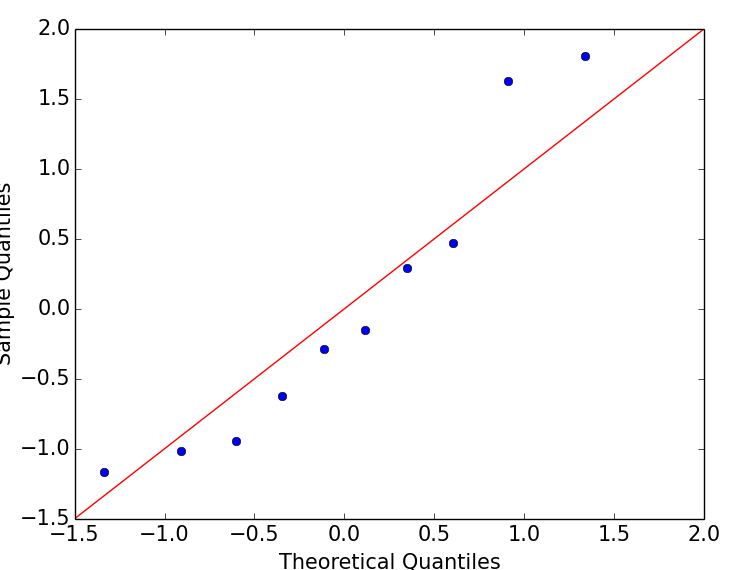
\includegraphics[width=\linewidth]{figs/normality/10samples_bootstrapping2.png}
\caption{Bootstrapping samples from Experiment E1} \label{fig:normality_bootstrapping}
\end{subfigure}
\caption[Normal Q-Q plot example]{Normal Q-Q plots generated by samples from a normal distribution, and from the baseline and curriculum population of Experiment E1 - 0\% omission noise. } \label{fig:normalityqq}
\end{figure}


\section{Increasing Levels of Random Noise Experiment}
\label{app:randomnoiseexperiment}
\todo[inline]{Do this}
\todo[inline]{Test loss figure for bootstrapping and baseline (confident if time allows}
\todo[inline]{Explain results.}
\todo[inline]{Noise illustration, random noise vs omission noise}

\pagebreak
\section{Road Detection Systems Results}
\label{app:roaddetectionresults}
In this appendix results from the best performing convolutional neural networks are displayed. The precision and recall breakeven point of the model trained on the Massachusetts Roads Dataset is 0.8627. Whereas, the breakeven point for the best model trained on the Norwegian Roads Dataset is 0.7620.

\begin{figure}[H]
\begin{subfigure}{0.23\textwidth}
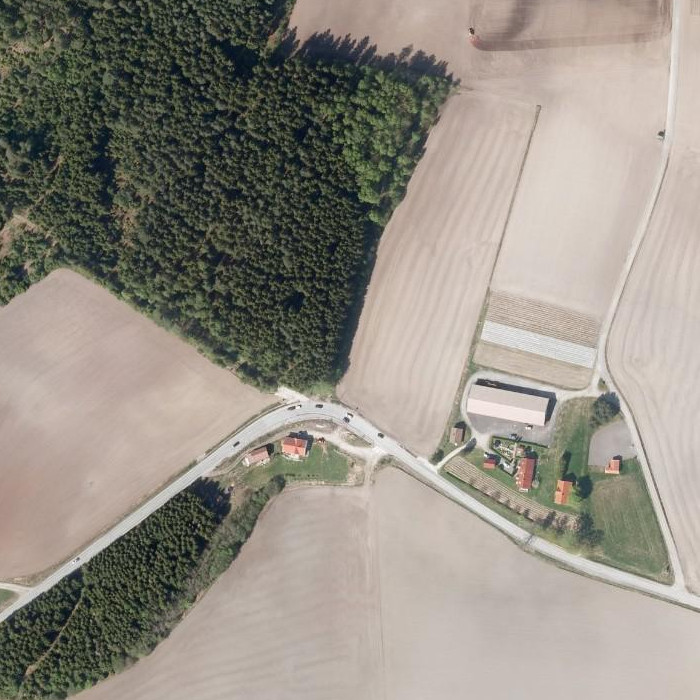
\includegraphics[width=\textwidth]{figs/appendix/img1151.jpg}
\caption{ Image. }
\vspace{0.1cm} % separation vertically between the subfigures
\end{subfigure}
\hspace*{\fill} % separation between the subfigures
\begin{subfigure}{0.23\textwidth}
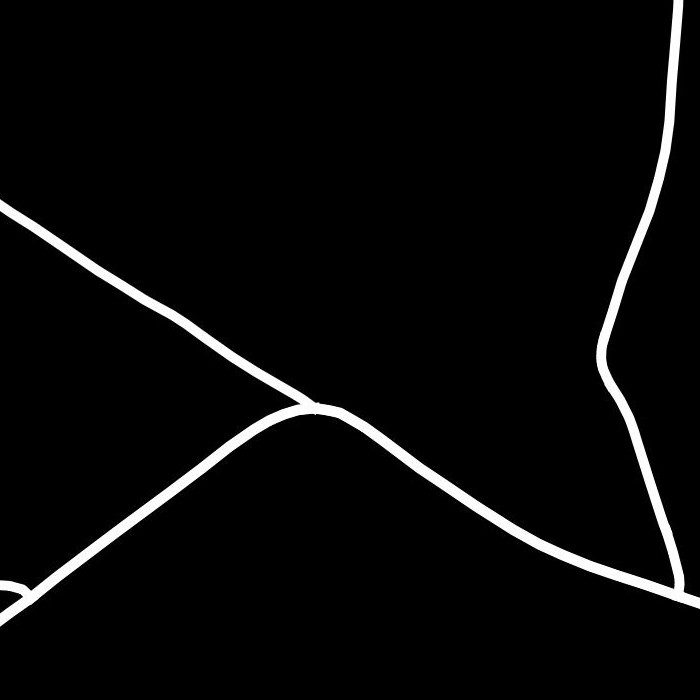
\includegraphics[width=\textwidth]{figs/appendix/label1151.jpg}
\caption{ Label. }
\vspace{0.1cm} % separation vertically between the subfigures
\end{subfigure}
\hspace*{\fill} % separation between the subfigures
\begin{subfigure}{0.23\textwidth}
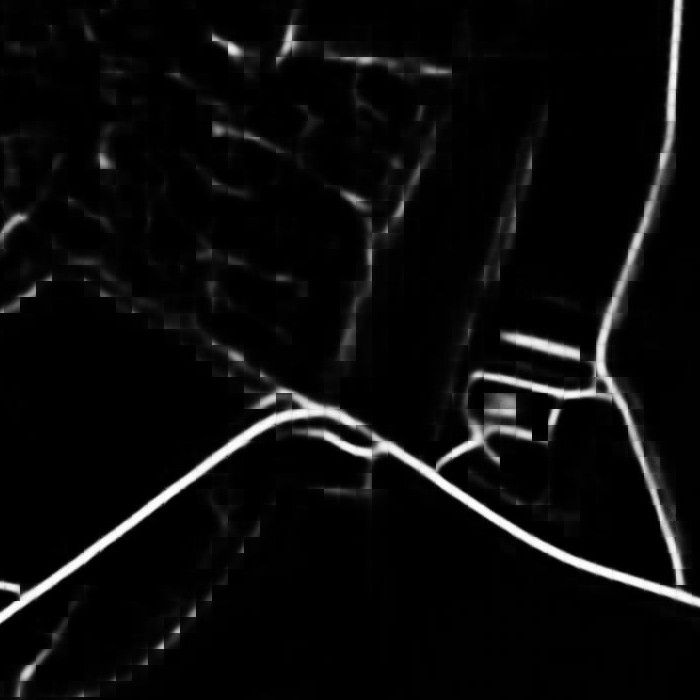
\includegraphics[width=\textwidth]{figs/appendix/pred1151.jpg}
\caption{ Prediction. }
\vspace{0.1cm} % separation vertically between the subfigures
\end{subfigure}
\hspace*{\fill} % separation between the subfigures
\begin{subfigure}{0.23\textwidth}
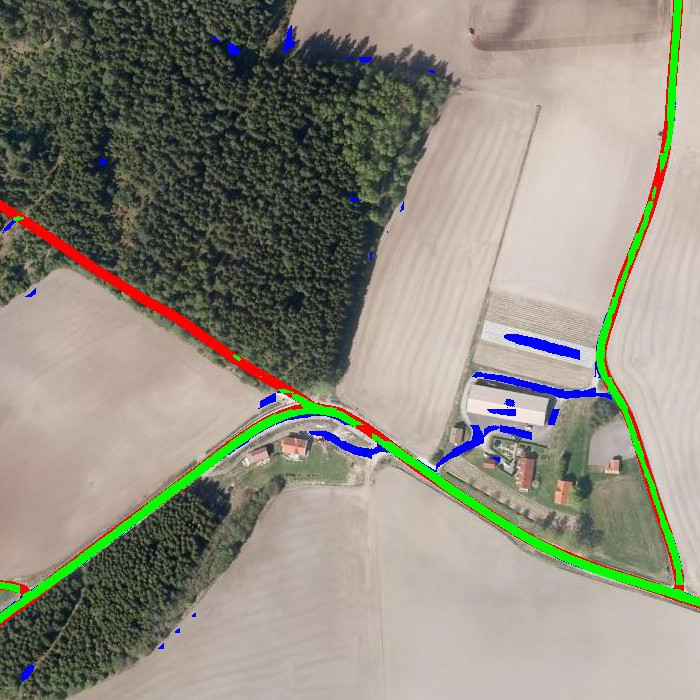
\includegraphics[width=\textwidth]{figs/appendix/hit1151.jpg}
\caption{ Hits. }
\vspace{0.1cm} % separation vertically between the subfigures
\end{subfigure}
\begin{subfigure}{0.23\textwidth}
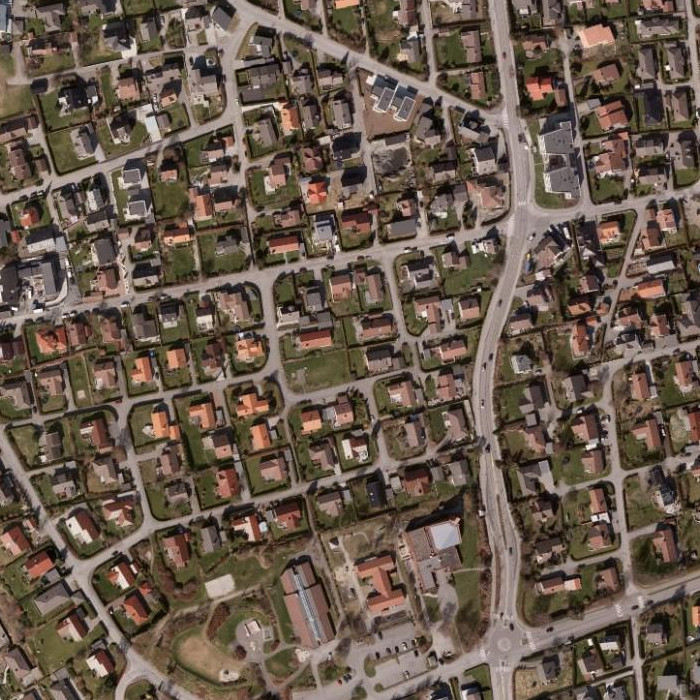
\includegraphics[width=\textwidth]{figs/appendix/img1160.jpg}
\caption{ Image.}
\vspace{0.1cm} % separation vertically between the subfigures
\end{subfigure}
\hspace*{\fill} % separation between the subfigures
\begin{subfigure}{0.23\textwidth}
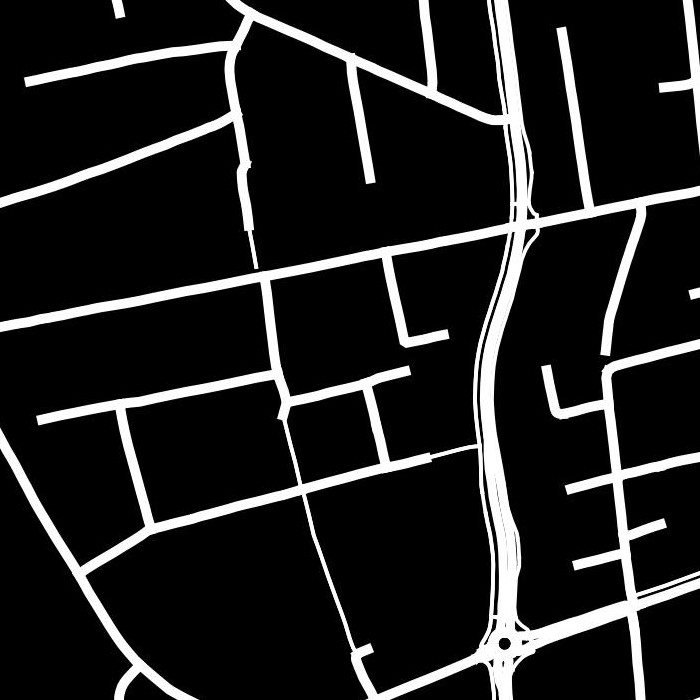
\includegraphics[width=\textwidth]{figs/appendix/label1160.jpg}
\caption{Label}
\vspace{0.1cm} % separation vertically between the subfigures
\end{subfigure}
\hspace*{\fill} % separation between the subfigures
\begin{subfigure}{0.23\textwidth}
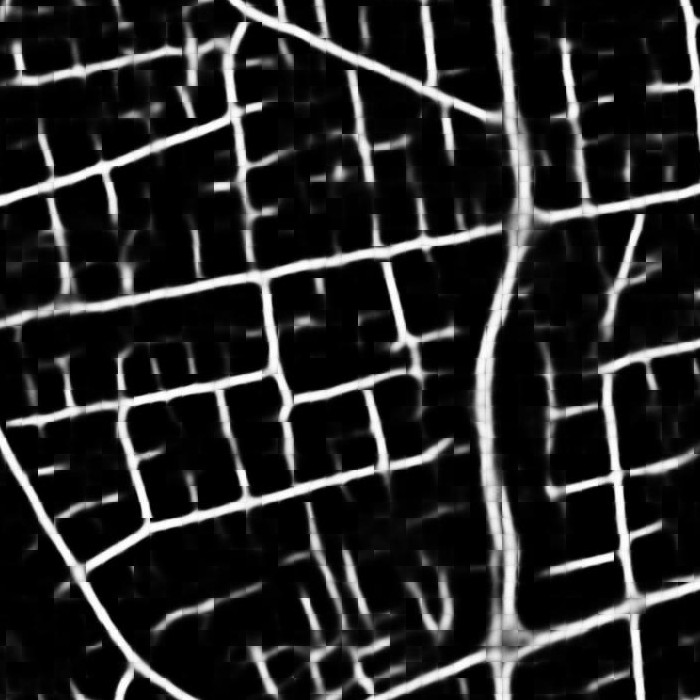
\includegraphics[width=\textwidth]{figs/appendix/pred1160.jpg}
\caption{Prediction.}
\vspace{0.1cm} % separation vertically between the subfigures
\end{subfigure}
\hspace*{\fill} % separation between the subfigures
\begin{subfigure}{0.23\textwidth}
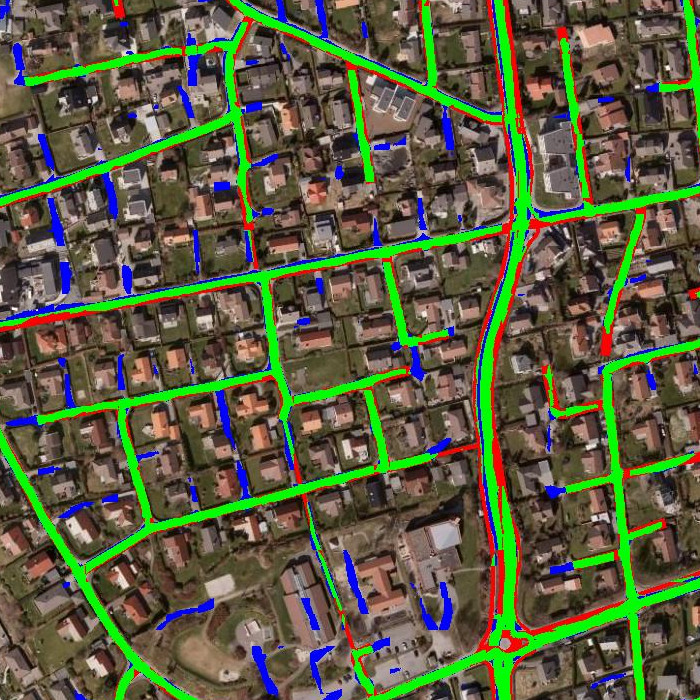
\includegraphics[width=\textwidth]{figs/appendix/hit1160.jpg}
\caption{Hits.}
\vspace{0.1cm} % separation vertically between the subfigures
\end{subfigure}
\begin{subfigure}{0.23\textwidth}
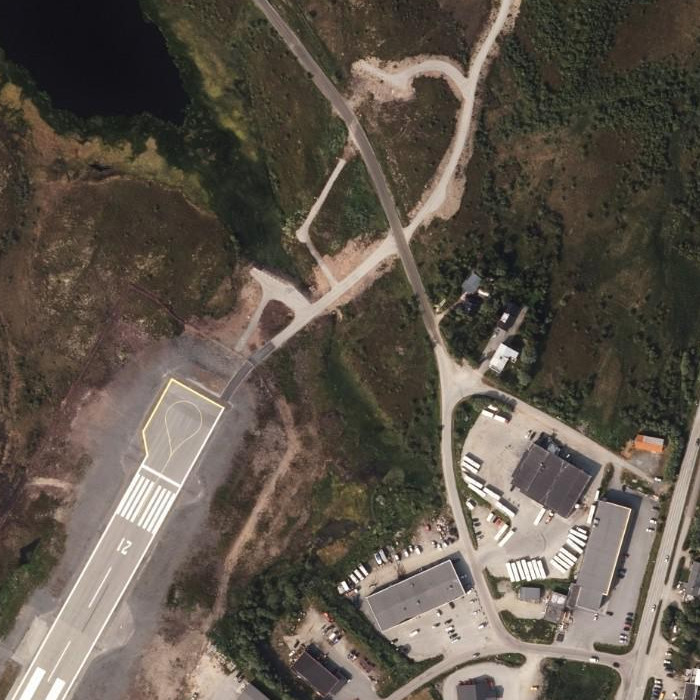
\includegraphics[width=\textwidth]{figs/appendix/img1205.jpg}
\caption{ Image. }
\vspace{0.1cm} % separation vertically between the subfigures
\end{subfigure}
\hspace*{\fill} % separation between the subfigures
\begin{subfigure}{0.23\textwidth}
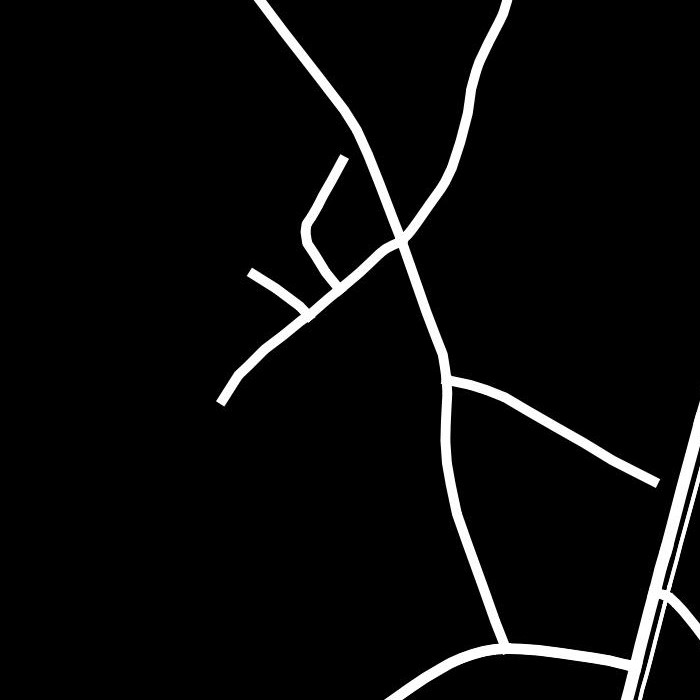
\includegraphics[width=\textwidth]{figs/appendix/label1205.jpg}
\caption{ Label. }
\vspace{0.1cm} % separation vertically between the subfigures
\end{subfigure}
\hspace*{\fill} % separation between the subfigures
\begin{subfigure}{0.23\textwidth}
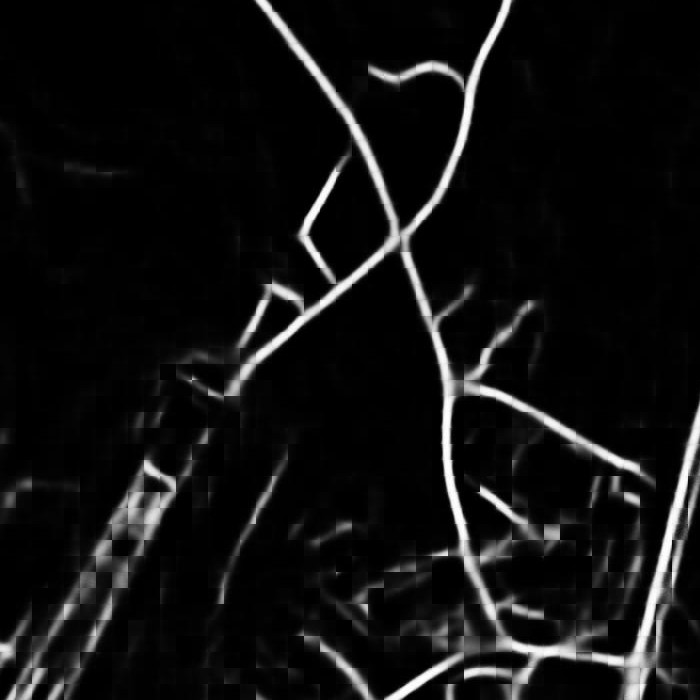
\includegraphics[width=\textwidth]{figs/appendix/pred1205.jpg}
\caption{ Prediction. }
\vspace{0.1cm} % separation vertically between the subfigures
\end{subfigure}
\hspace*{\fill} % separation between the subfigures
\begin{subfigure}{0.23\textwidth}
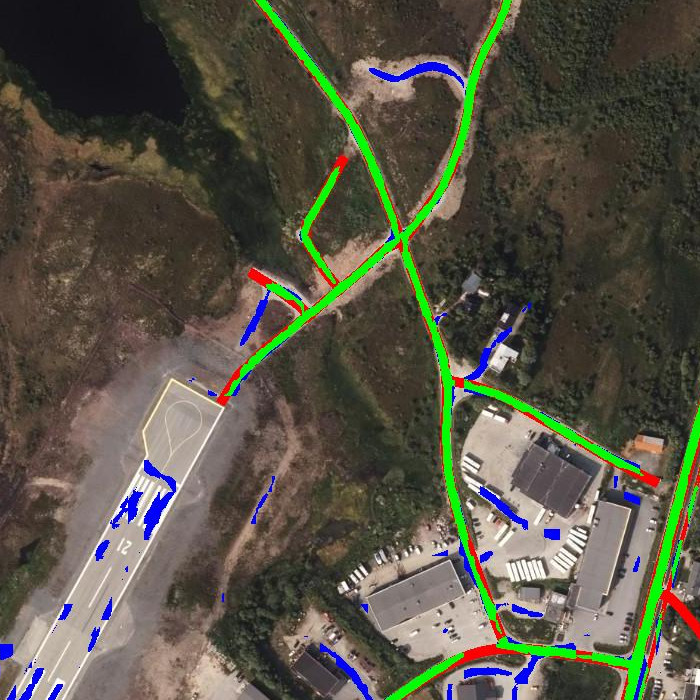
\includegraphics[width=\textwidth]{figs/appendix/hit1205.jpg}
\caption{ Hits. }
\vspace{0.1cm} % separation vertically between the subfigures
\end{subfigure}
\begin{subfigure}{0.23\textwidth}
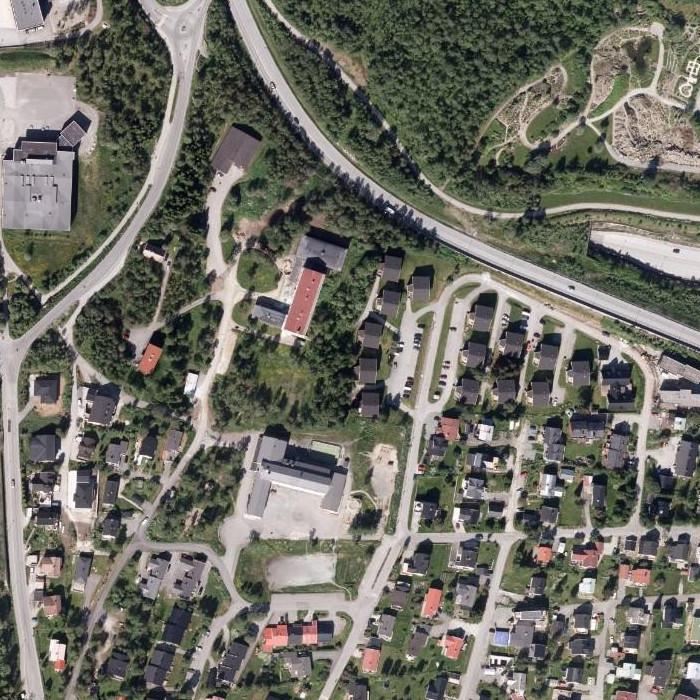
\includegraphics[width=\textwidth]{figs/appendix/img1217.jpg}
\caption{ Image.}
\vspace{0.1cm} % separation vertically between the subfigures
\end{subfigure}
\hspace*{\fill} % separation between the subfigures
\begin{subfigure}{0.23\textwidth}
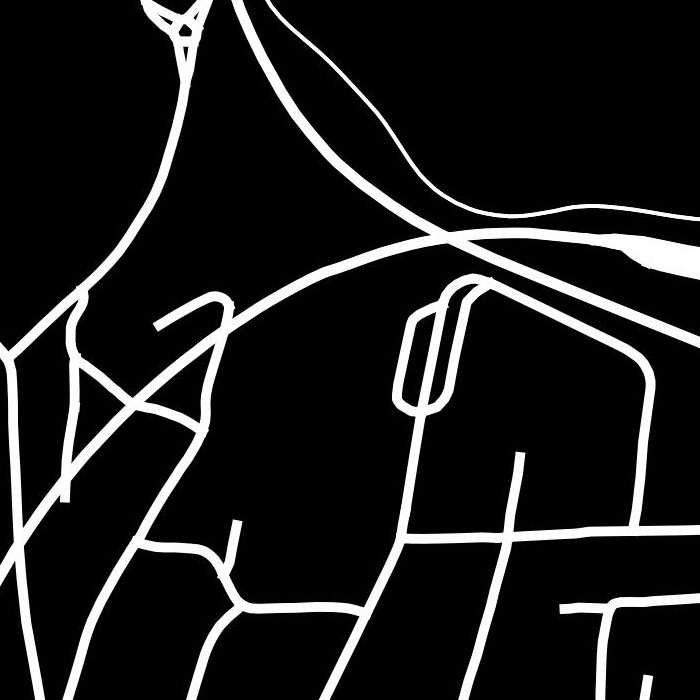
\includegraphics[width=\textwidth]{figs/appendix/label1217.jpg}
\caption{Label}
\vspace{0.1cm} % separation vertically between the subfigures
\end{subfigure}
\hspace*{\fill} % separation between the subfigures
\begin{subfigure}{0.23\textwidth}
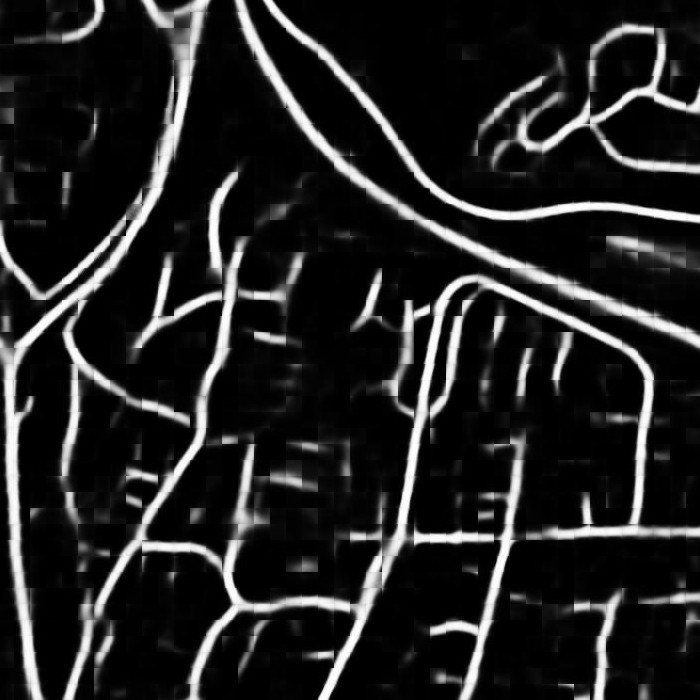
\includegraphics[width=\textwidth]{figs/appendix/pred1217.jpg}
\caption{Prediction.}
\vspace{0.1cm} % separation vertically between the subfigures
\end{subfigure}
\hspace*{\fill} % separation between the subfigures
\begin{subfigure}{0.23\textwidth}
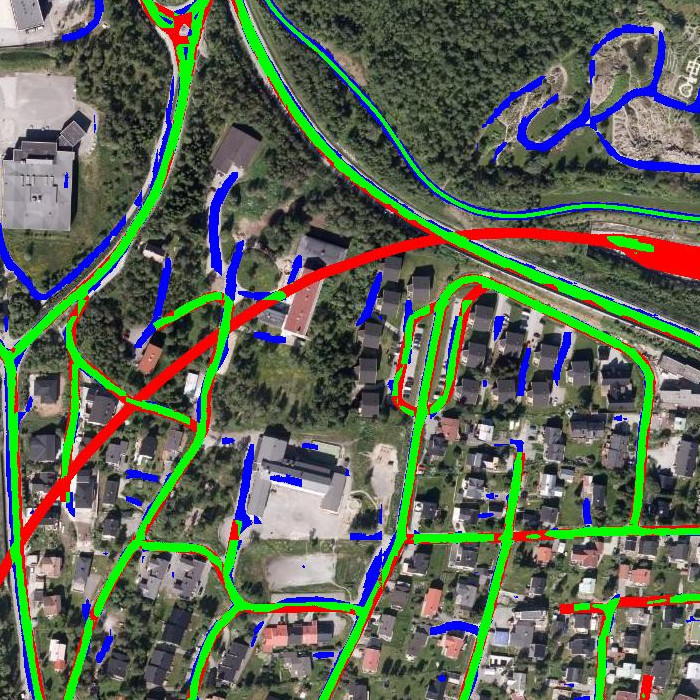
\includegraphics[width=\textwidth]{figs/appendix/hit1217.jpg}
\caption{Hits.}
\vspace{0.1cm} % separation vertically between the subfigures
\end{subfigure}
\vspace{-1\baselineskip}
\caption[Norway Road extraction results]{Road extraction results from the Norwegian Roads Dataset.} \label{fig:Norway_app_results2}
\end{figure}

\begin{figure}[H]
\begin{subfigure}{0.23\textwidth}
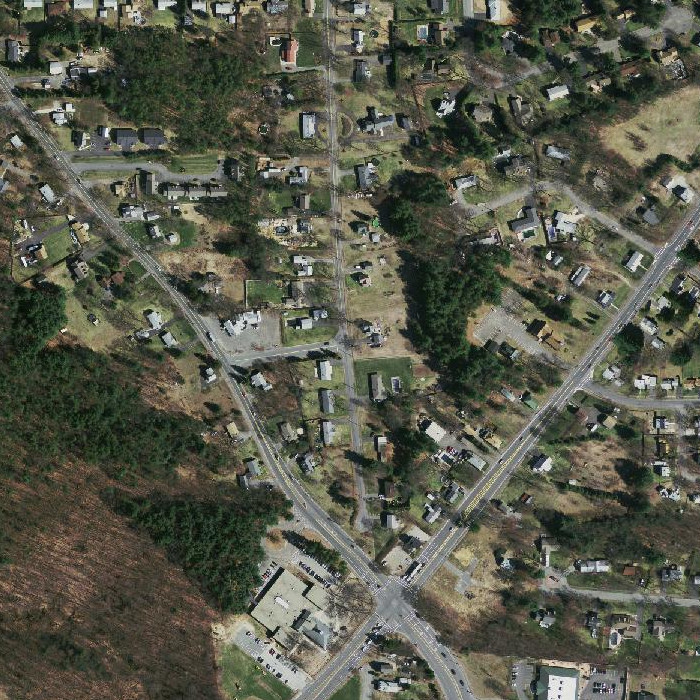
\includegraphics[width=\textwidth]{figs/appendix/img11128870_15.jpg}
\caption{ Image. }
\vspace{0.2cm} % separation vertically between the subfigures
\end{subfigure}
\hspace*{\fill} % separation between the subfigures
\begin{subfigure}{0.23\textwidth}
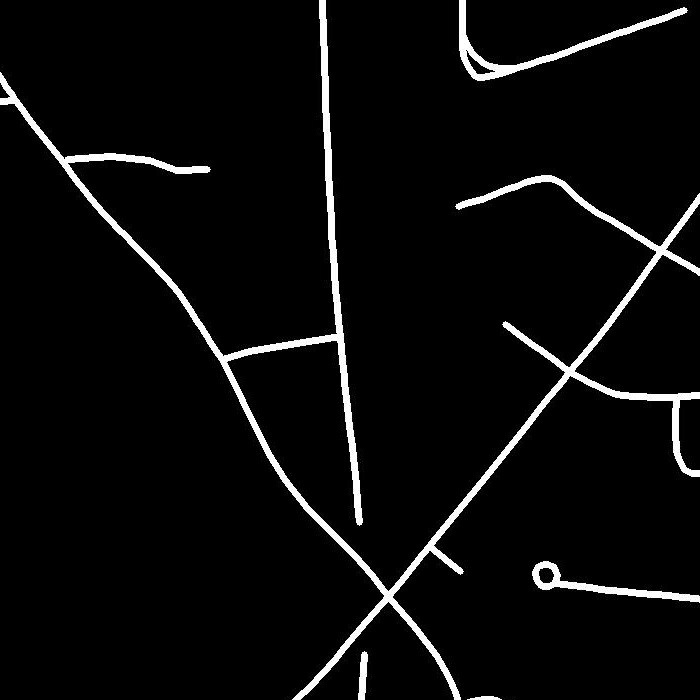
\includegraphics[width=\textwidth]{figs/appendix/label11128870_15.jpg}
\caption{ Label. }
\vspace{0.2cm} % separation vertically between the subfigures
\end{subfigure}
\hspace*{\fill} % separation between the subfigures
\begin{subfigure}{0.23\textwidth}
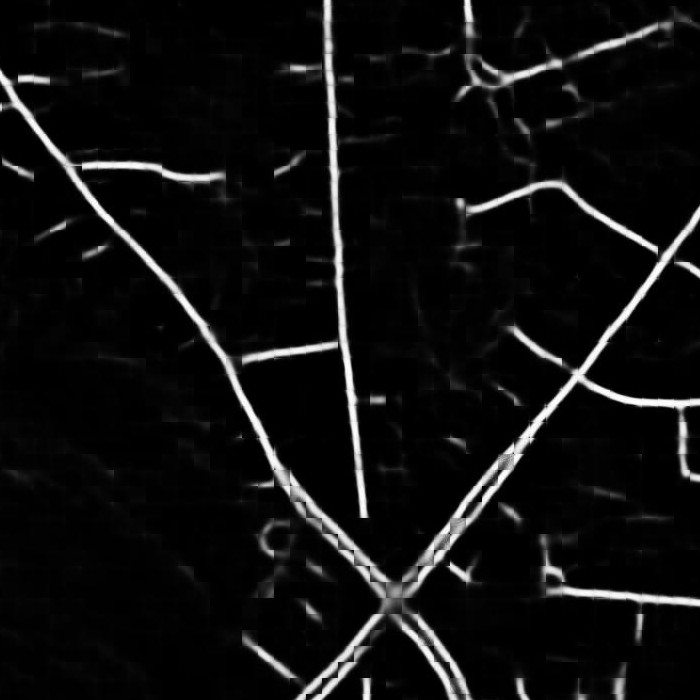
\includegraphics[width=\textwidth]{figs/appendix/pred11128870_15.jpg}
\caption{ Prediction. }
\vspace{0.2cm} % separation vertically between the subfigures
\end{subfigure}
\hspace*{\fill} % separation between the subfigures
\begin{subfigure}{0.23\textwidth}
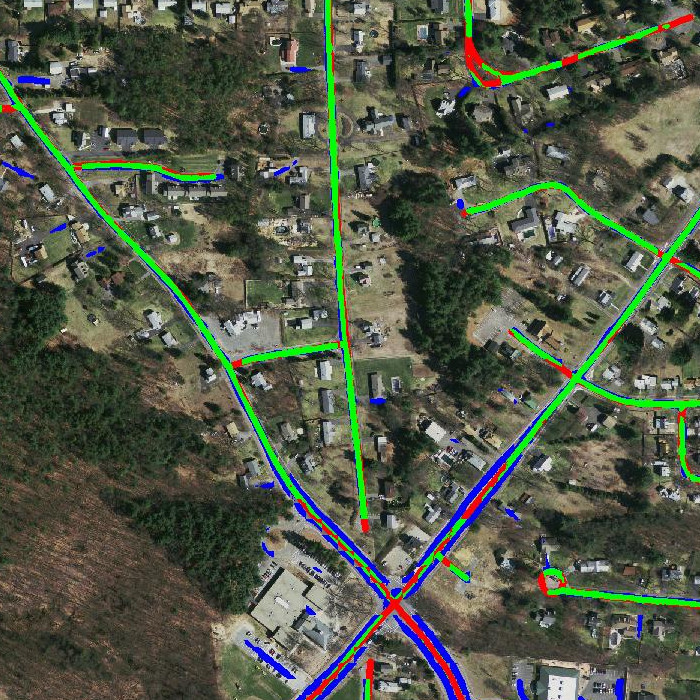
\includegraphics[width=\textwidth]{figs/appendix/hit11128870_15.jpg}
\caption{ Hits. }
\vspace{0.2cm} % separation vertically between the subfigures
\end{subfigure}
\begin{subfigure}{0.23\textwidth}
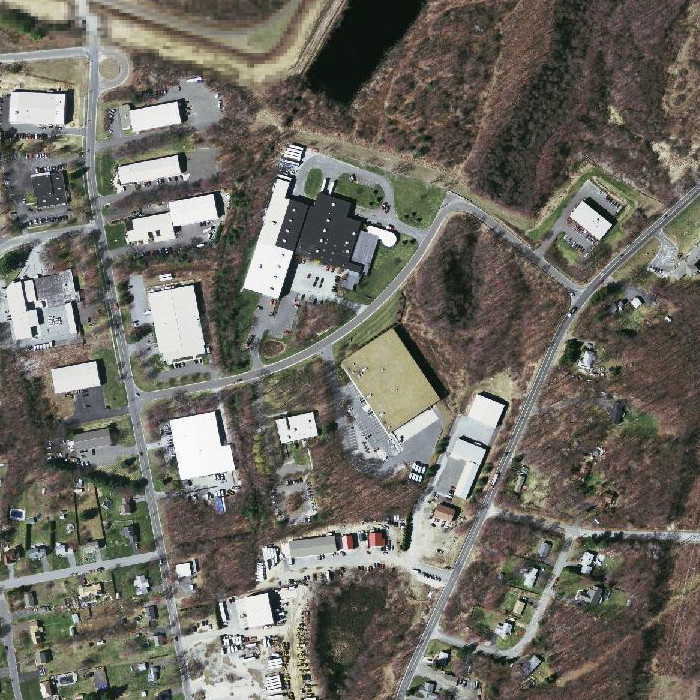
\includegraphics[width=\textwidth]{figs/appendix/img11728825_15.jpg}
\caption{ Image.}
\vspace{0.2cm} % separation vertically between the subfigures
\end{subfigure}
\hspace*{\fill} % separation between the subfigures
\begin{subfigure}{0.23\textwidth}
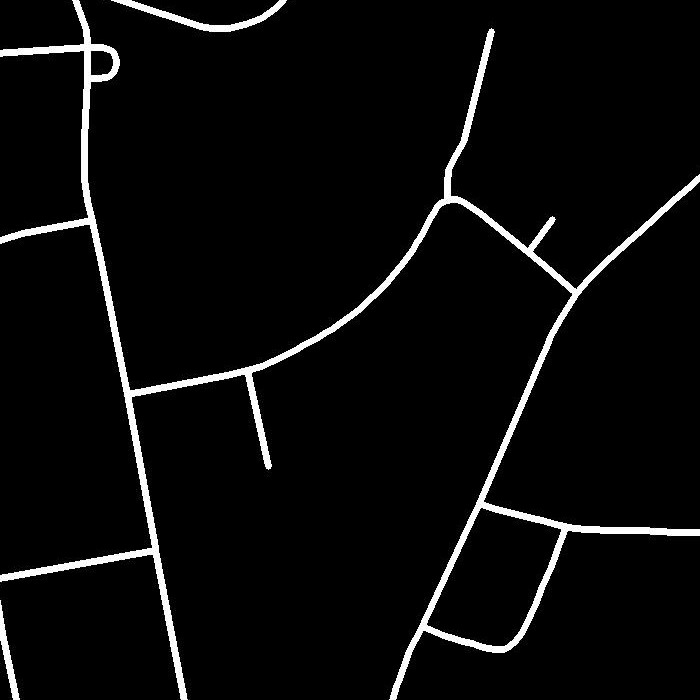
\includegraphics[width=\textwidth]{figs/appendix/label11728825_15.jpg}
\caption{Label}
\vspace{0.2cm} % separation vertically between the subfigures
\end{subfigure}
\hspace*{\fill} % separation between the subfigures
\begin{subfigure}{0.23\textwidth}
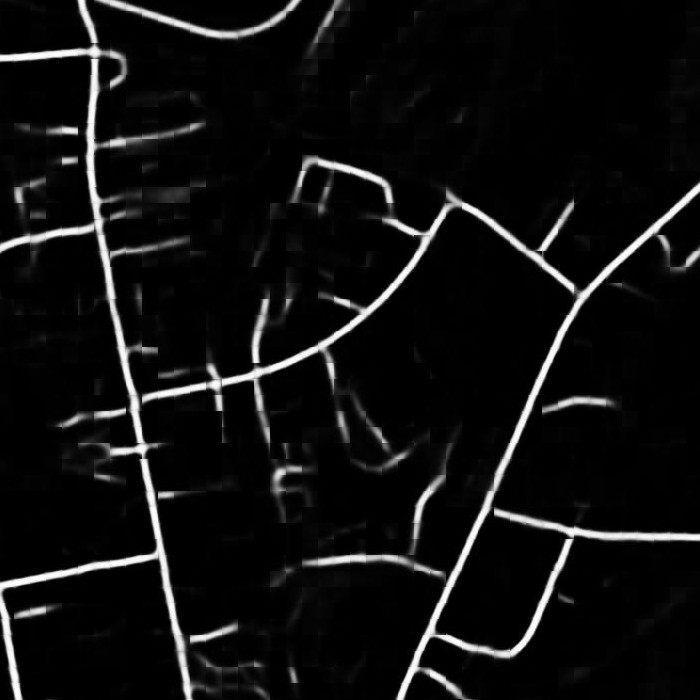
\includegraphics[width=\textwidth]{figs/appendix/pred11728825_15.jpg}
\caption{Prediction.}
\vspace{0.2cm} % separation vertically between the subfigures
\end{subfigure}
\hspace*{\fill} % separation between the subfigures
\begin{subfigure}{0.23\textwidth}
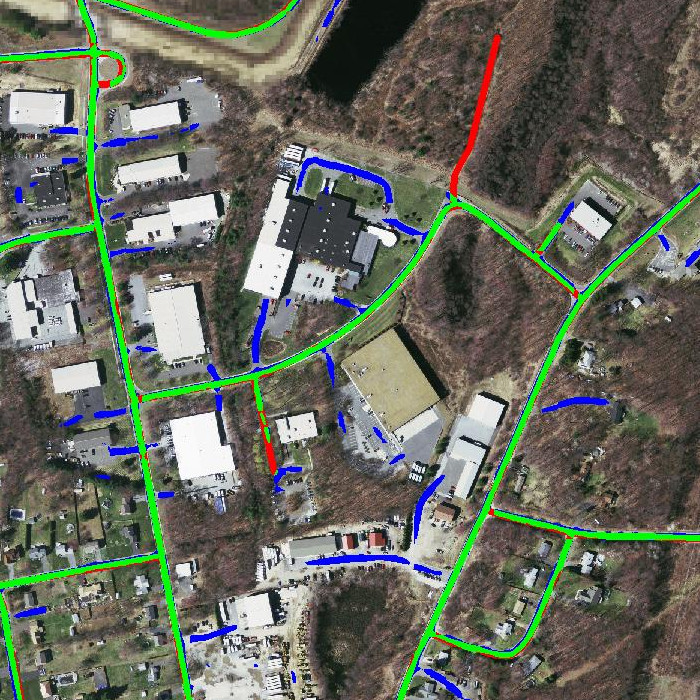
\includegraphics[width=\textwidth]{figs/appendix/hit11728825_15.jpg}
\caption{Hits.}
\vspace{0.2cm} % separation vertically between the subfigures
\end{subfigure}
\begin{subfigure}{0.23\textwidth}
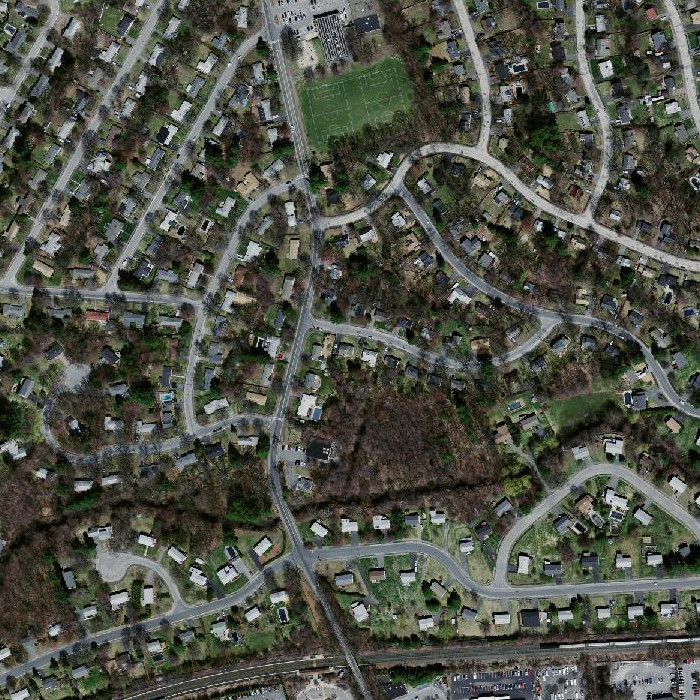
\includegraphics[width=\textwidth]{figs/appendix/img20878930_15.jpg}
\caption{ Image. }
\vspace{0.2cm} % separation vertically between the subfigures
\end{subfigure}
\hspace*{\fill} % separation between the subfigures
\begin{subfigure}{0.23\textwidth}
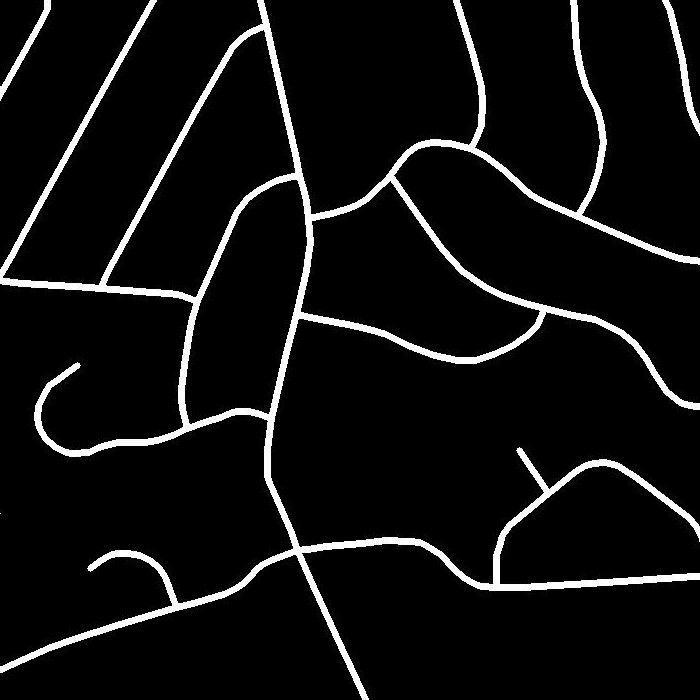
\includegraphics[width=\textwidth]{figs/appendix/label20878930_15.jpg}
\caption{ Label. }
\vspace{0.2cm} % separation vertically between the subfigures
\end{subfigure}
\hspace*{\fill} % separation between the subfigures
\begin{subfigure}{0.23\textwidth}
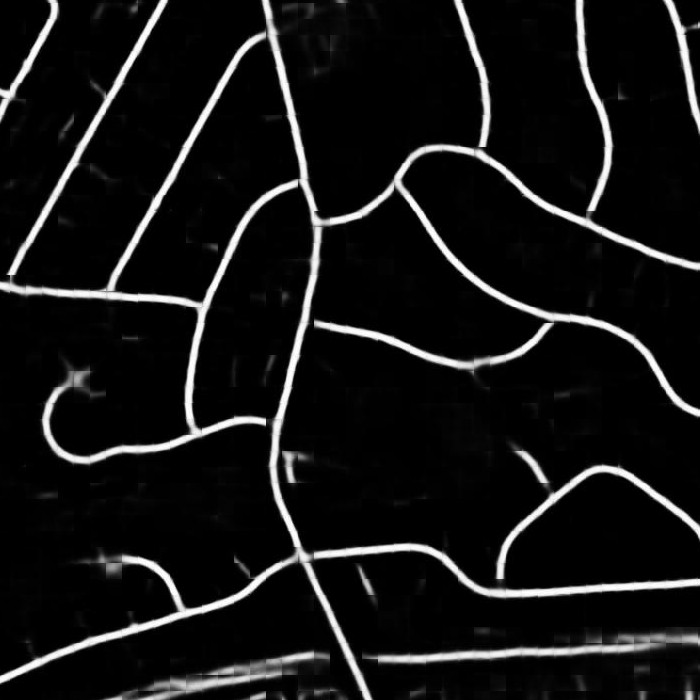
\includegraphics[width=\textwidth]{figs/appendix/pred20878930_15.jpg}
\caption{ Prediction. }
\vspace{0.2cm} % separation vertically between the subfigures
\end{subfigure}
\hspace*{\fill} % separation between the subfigures
\begin{subfigure}{0.23\textwidth}
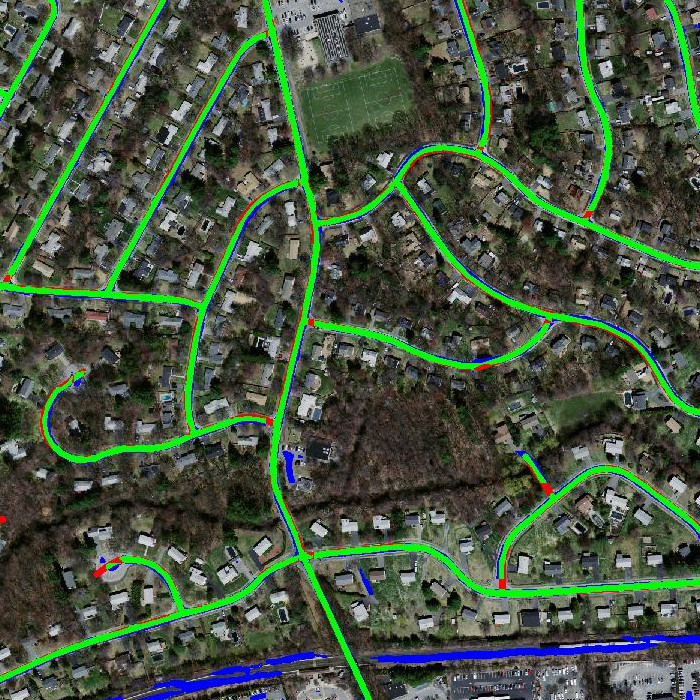
\includegraphics[width=\textwidth]{figs/appendix/hit20878930_15.jpg}
\caption{ Hits. }
\vspace{0.2cm} % separation vertically between the subfigures
\end{subfigure}
\begin{subfigure}{0.23\textwidth}
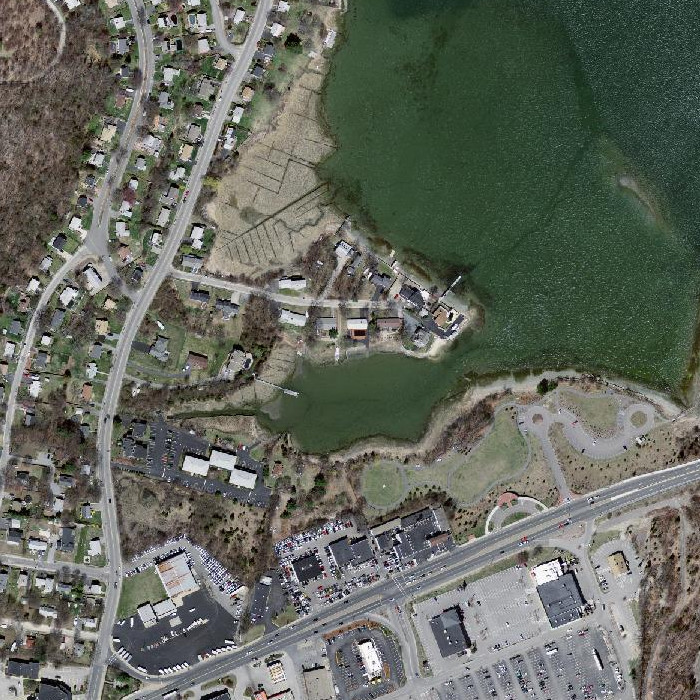
\includegraphics[width=\textwidth]{figs/appendix/img24628885_15.jpg}
\caption{ Image.}
\vspace{0.2cm} % separation vertically between the subfigures
\end{subfigure}
\hspace*{\fill} % separation between the subfigures
\begin{subfigure}{0.23\textwidth}
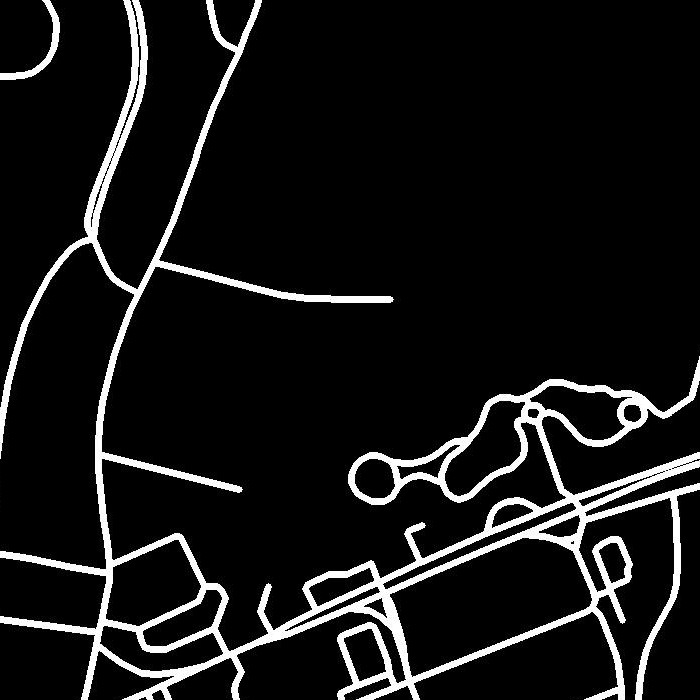
\includegraphics[width=\textwidth]{figs/appendix/label24628885_15.jpg}
\caption{Label}
\vspace{0.2cm} % separation vertically between the subfigures
\end{subfigure}
\hspace*{\fill} % separation between the subfigures
\begin{subfigure}{0.23\textwidth}
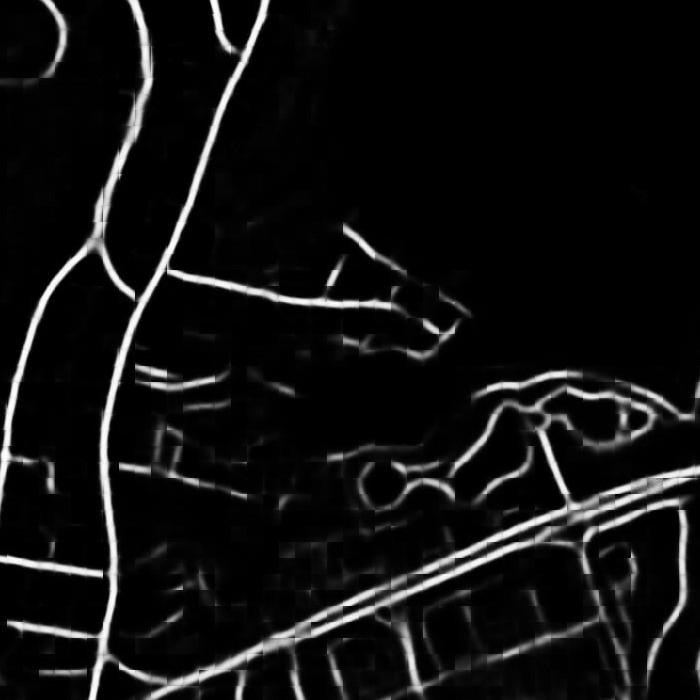
\includegraphics[width=\textwidth]{figs/appendix/pred24628885_15.jpg}
\caption{Prediction.}
\vspace{0.2cm} % separation vertically between the subfigures
\end{subfigure}
\hspace*{\fill} % separation between the subfigures
\begin{subfigure}{0.23\textwidth}
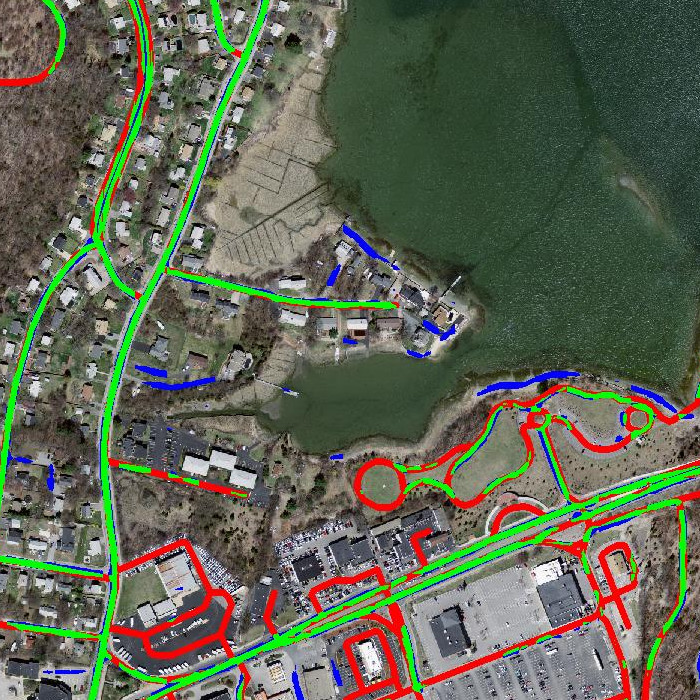
\includegraphics[width=\textwidth]{figs/appendix/hit24628885_15.jpg}
\caption{Hits.}
\vspace{0.2cm} % separation vertically between the subfigures
\end{subfigure}
\vspace{-1\baselineskip}
\caption[Massachusetts Road extraction results]{Road extraction results from the Massachusetts Roads Dataset.} \label{fiMass_app_results2}
\end{figure}

\pagebreak
\section{Experiment E2 Results}
\label{app:fullE5results}
The results from Experiment E2 were summarised by plotting the final test loss and precision and breakeven point for increasing levels of omission noise. In this appendix, the test loss figures for every noise rate is shown in Figure \ref{fig:E2_all_lc}, while the precision and recall curve figures are depicted in Figure \ref{fig:E2_all_pr}.
\begin{figure}[H]
\begin{subfigure}{0.31\textwidth}
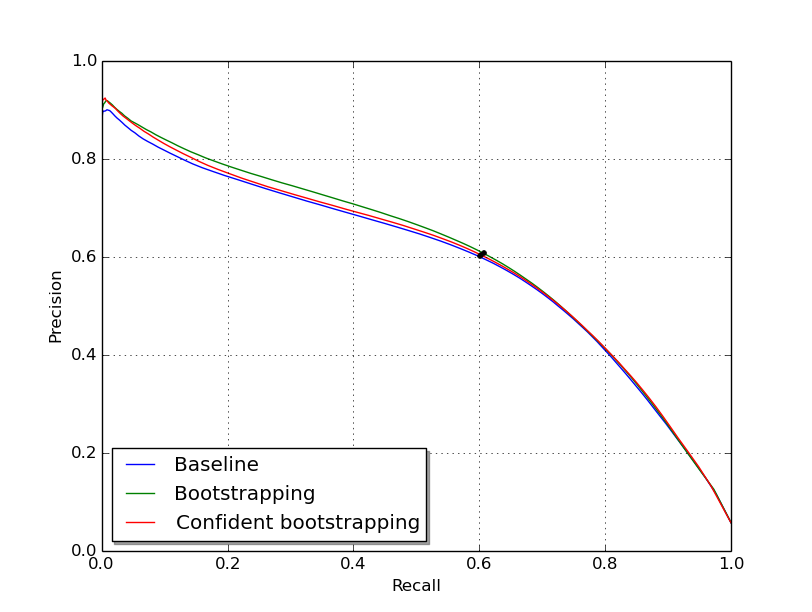
\includegraphics[width=\textwidth]{figs/E2/pr_0.png}
\caption{ 0\% } \label{fig:app_E2_0_pr}
\vspace{-0.1cm} % separation vertically between the subfigures
\end{subfigure}
\hspace*{\fill} % separation between the subfigures
\begin{subfigure}{0.31\textwidth}
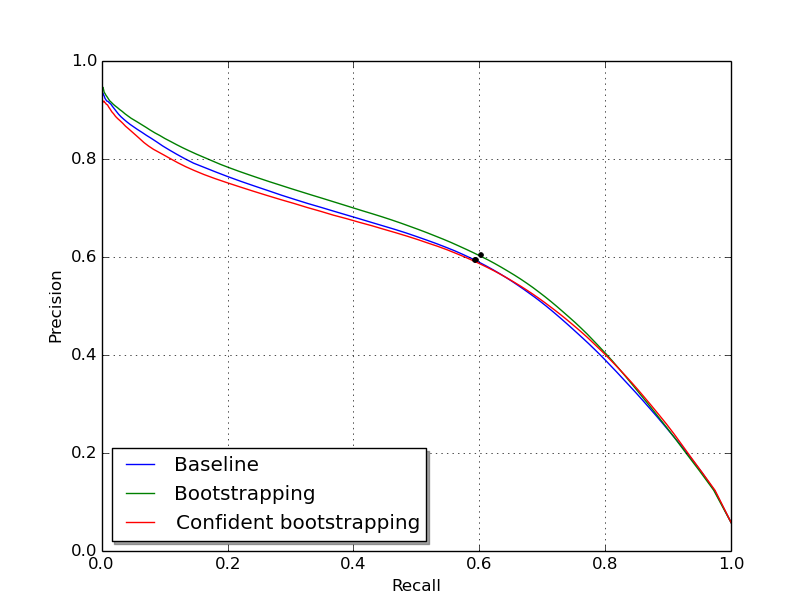
\includegraphics[width=\textwidth]{figs/E2/pr_1.png}
\caption{10\% } \label{fig:app_E2_1_pr}
\vspace{-0.1cm} % separation vertically between the subfigures
\end{subfigure}
\hspace*{\fill} % separation between the subfigures
\begin{subfigure}{0.31\textwidth}
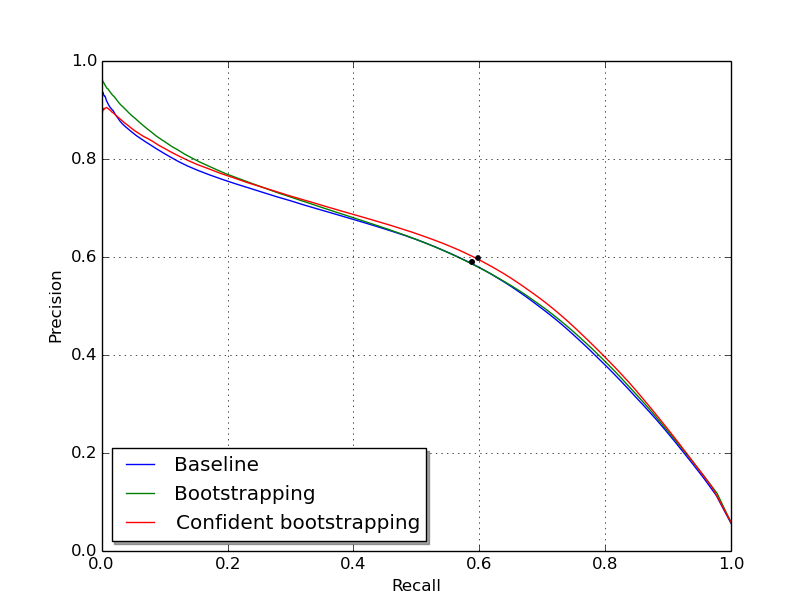
\includegraphics[width=\textwidth]{figs/E2/pr_2.png}
\caption{20\% } \label{fig:app_E2_2_pr}
\vspace{-0.1cm} % separation vertically between the subfigures
\end{subfigure}
\begin{subfigure}{0.31\textwidth}
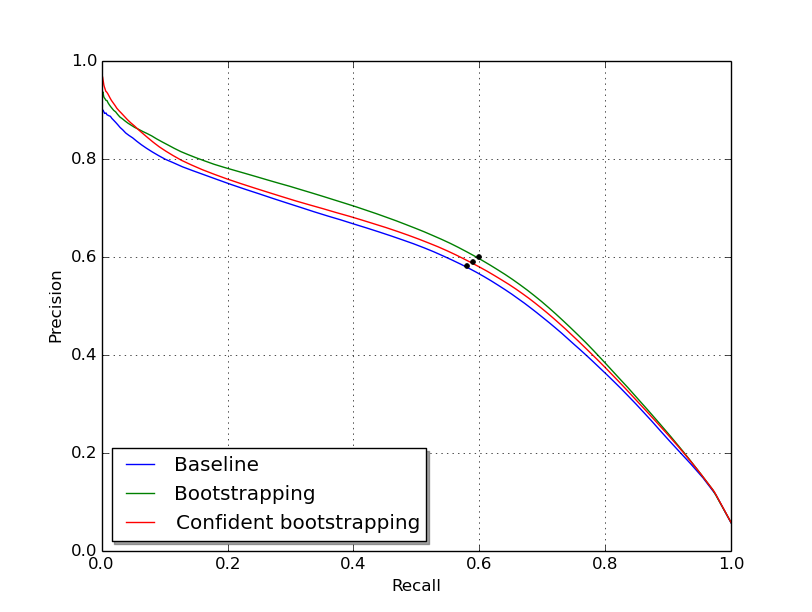
\includegraphics[width=\textwidth]{figs/E2/pr_3.png}
\caption{ 30\%} \label{fig:app_E2_3_pr}
\vspace{-0.1cm} % separation vertically between the subfigures
\end{subfigure}
\hspace*{\fill} % separation between the subfigures
\begin{subfigure}{0.31\textwidth}
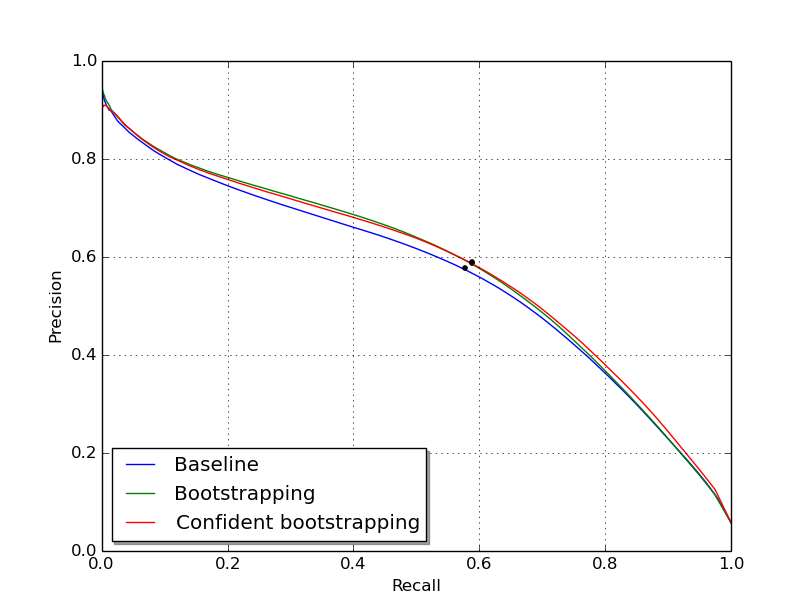
\includegraphics[width=\textwidth]{figs/E2/pr_4.png}
\caption{40\%} \label{fig:app_E2_4_pr}
\vspace{-0.1cm} % separation vertically between the subfigures
\end{subfigure}
\vspace{-0.6\baselineskip}
\caption{E2 - Precision and recall plot for several levels of omission noise.} \label{fig:E2_all_pr}
\end{figure}
\vspace{-0.7cm}
\begin{figure}[H]
\begin{subfigure}{0.3\textwidth}
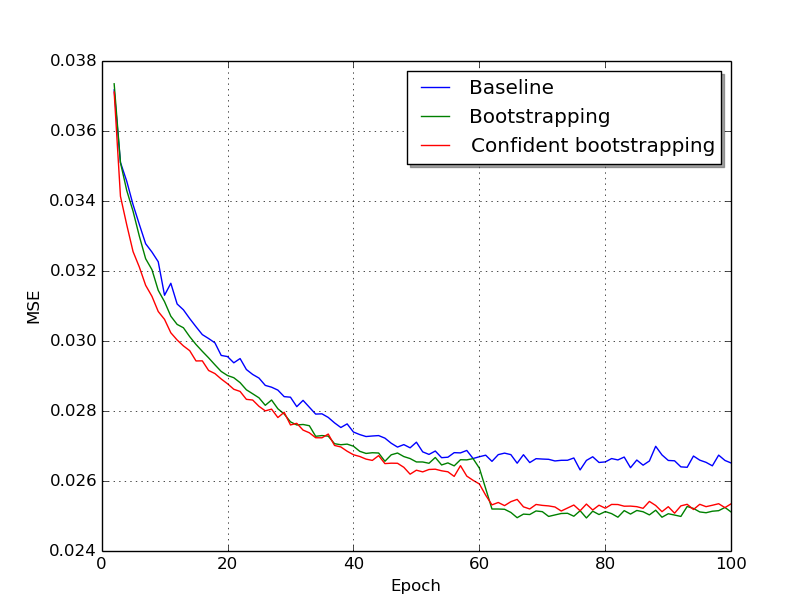
\includegraphics[width=\textwidth]{figs/E2/lc_0.png}
\caption{ 0\% } \label{fig:app_E2_0_lc}
\vspace{-0.1cm} % separation vertically between the subfigures
\end{subfigure}
\hspace*{\fill} % separation between the subfigures
\begin{subfigure}{0.31\textwidth}
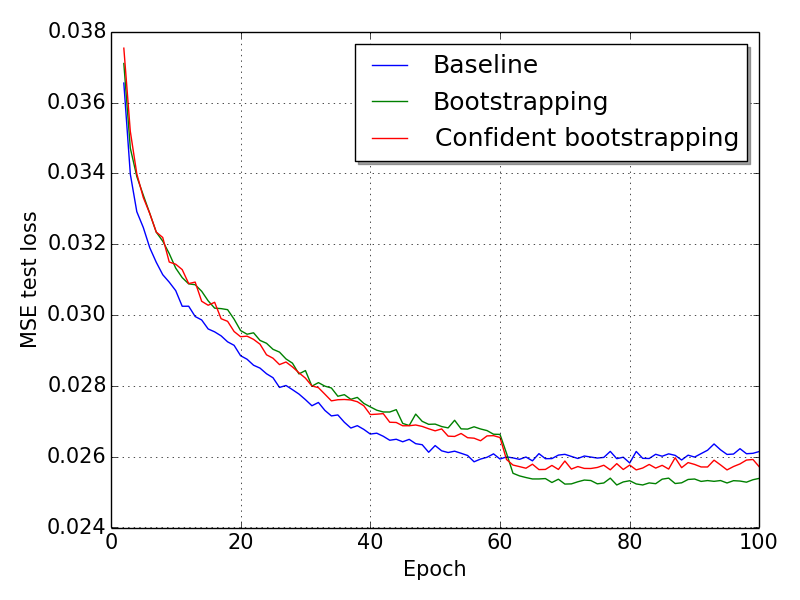
\includegraphics[width=\textwidth]{figs/E2/lc_1.png}
\caption{10\% } \label{fig:app_E2_1_lc}
\vspace{-0.1cm} % separation vertically between the subfigures
\end{subfigure}
\hspace*{\fill} % separation between the subfigures
\begin{subfigure}{0.31\textwidth}
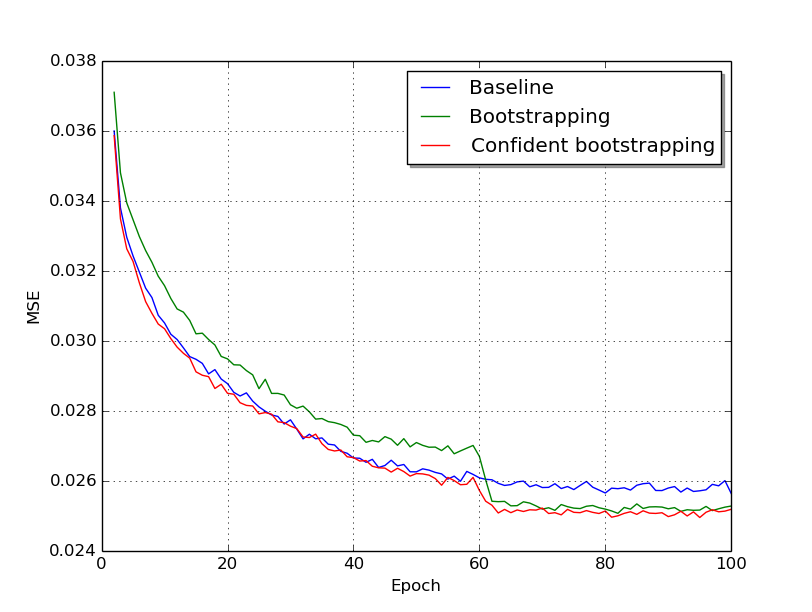
\includegraphics[width=\textwidth]{figs/E2/lc_2.png}
\caption{20\% } \label{fig:app_E2_2_lc}
\vspace{-0.1cm} % separation vertically between the subfigures
\end{subfigure}
\begin{subfigure}{0.31\textwidth}
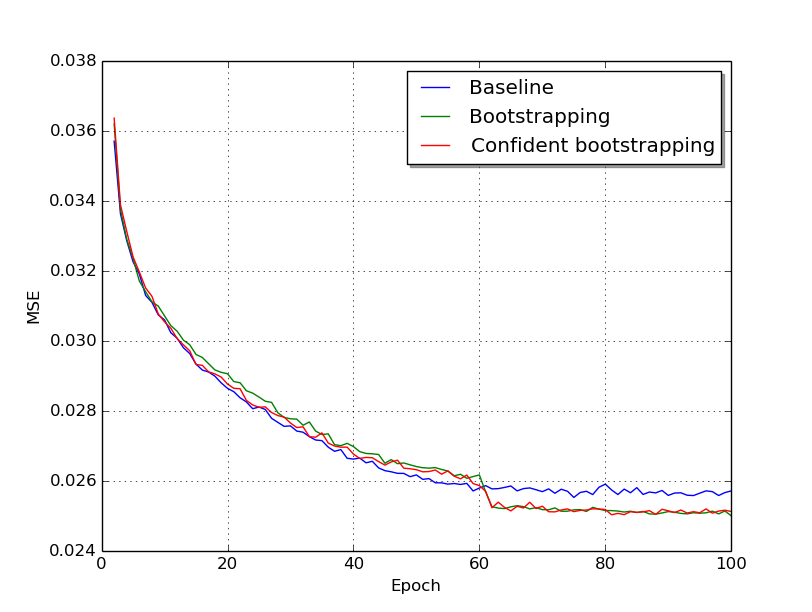
\includegraphics[width=\textwidth]{figs/E2/lc_3.png}
\caption{ 30\%} \label{fig:app_E2_3_lc}
\vspace{-0.1cm} % separation vertically between the subfigures
\end{subfigure}
\hspace*{\fill} % separation between the subfigures
\begin{subfigure}{0.31\textwidth}
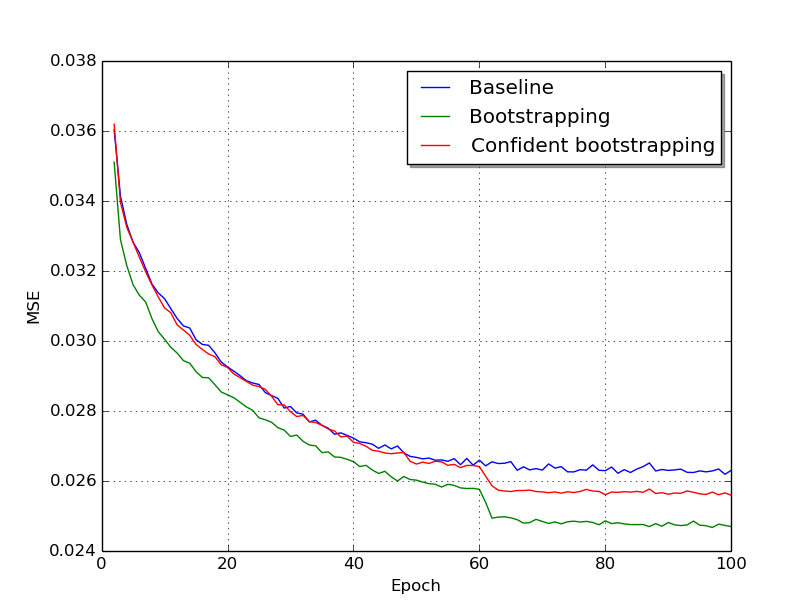
\includegraphics[width=\textwidth]{figs/E2/lc_4.png}
\caption{40\%} \label{fig:app_E2_4_lc}
\vspace{-0.1cm} % separation vertically between the subfigures
\end{subfigure}
\vspace{-0.6\baselineskip}
\caption{E2 - Test loss comparisons for several levels of omission noise.} \label{fig:E2_all_lc}
\end{figure}


\section{TODOs which apply to entire thesis}
\todo[inline]{Remove this part!}
\begin{itemize}
\item proof read (second time, and be vary of incorrect tense. Also look out for long sentences, and tedious language. If used is used to often, make some fixes here as well)
\item Ensure either by a footnote or something that road extraction and road detection and so forth is the same thing
\item What does harder examples look like? Examples
\item Example of road removal first paragraph Section 4.3.1, Maybe in appendix?
\item organize with s because of british english?
\item Appendix for other results? Random noise results? 

\item Road extraction, road detection, semantic segmentation, patch-based. That they are the same thing needs to be integrated somewhere
\item Check that installation guides, or should they be removed because of length. They are in repositories so.. and dependencies are correct - Appendix A, B, C
\end{itemize}
